% A mindmap showing TeX online projects supported
% by DANTE e.V. which sponsors their server costs.
% Author: Stefan Kottwitz
\documentclass[border=10pt]{standalone}
%%%<
\usepackage{verbatim}
%%%>
%\begin{comment}
%:Title: Hindernisvermeidung
%:Tags: Mindmaps
%:Author: Tino Krueger-Basjmeleh
%
%\end{comment}
\usepackage[utf8]{inputenc}
%\usepackage{dtklogos}
\usepackage{tikz}
\usetikzlibrary{mindmap,shadows}
\usepackage[hidelinks,pdfencoding=auto]{hyperref}
% Information boxes
\newcommand*{\info}[4][16.3]{%
  \node [ annotation, #3, scale=0.65, text width = #1em,
          inner sep = 2mm ] at (#2) {%
  \list{$\bullet$}{\topsep=0pt\itemsep=0pt\parsep=0pt
    \parskip=0pt\labelwidth=8pt\leftmargin=8pt
    \itemindent=0pt\labelsep=2pt}%
    #4
  \endlist
  };
}


\definecolor{ifptgray}{RGB}{128,128,128}
\definecolor{ifptorange}{RGB}{252,148,28}
\definecolor{ifptred}{RGB}{162,0,0}
\definecolor{ifptgreen}{RGB}{118,205,3}
\definecolor{ifptblue}{RGB}{23,131,232}
\definecolor{ifptdarkblue}{RGB}{2,38,110}
\definecolor{ifptlightblue}{RGB}{185,208,241}
\begin{document}
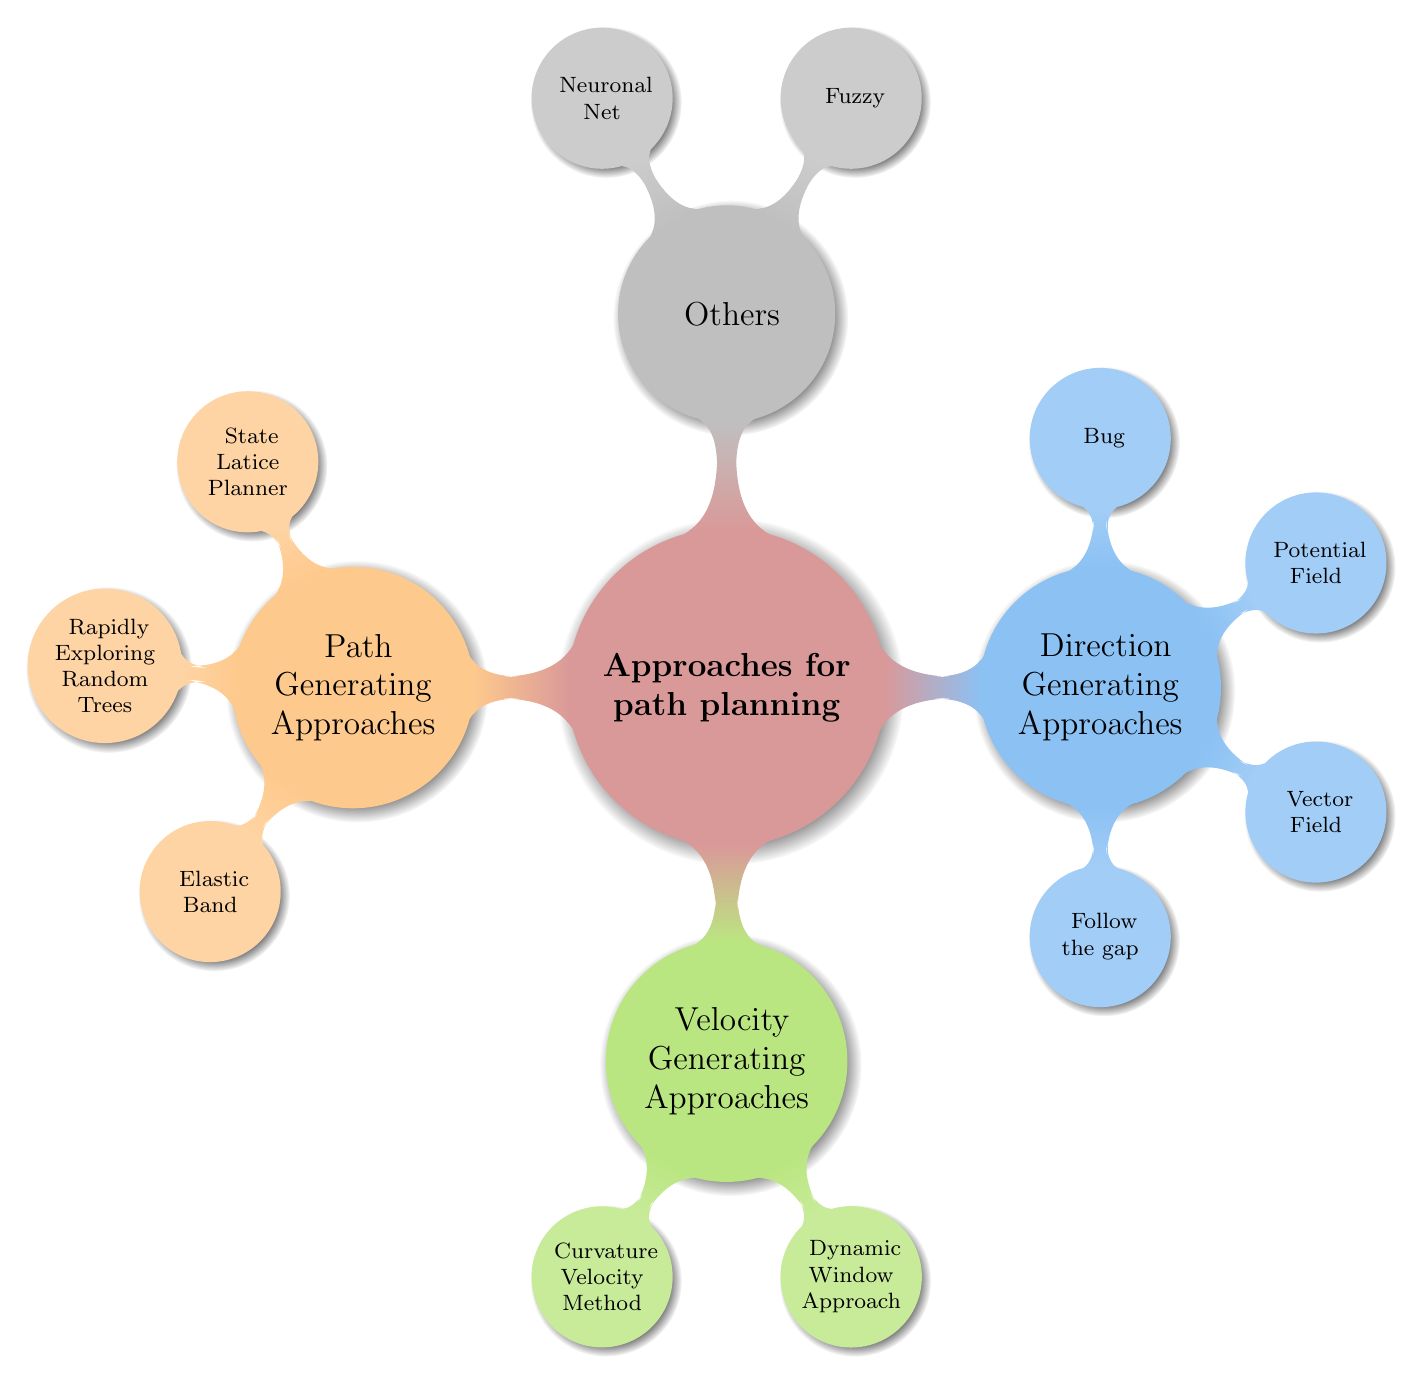
\begin{tikzpicture}[ every annotation/.style = {draw,
                     fill = white, font = \Large}]
  \path[mindmap,concept color=ifptred!40,text=black,
    every node/.style={concept,circular drop shadow},
    root/.style    = {concept color=ifptred!40,
      font=\large\bfseries,text width=10em},
    level 1 concept/.append style={ font = \large, sibling angle=90,text width=7.7em,
    level distance=13.5em,inner sep=0pt},
    level 2 concept/.append style={level distance=9em},
  ]
  node[root] {Approaches for \\
              path planning} [clockwise from=0]
    child[concept color=ifptblue!50] {
      node(Richtungsgenerierend) {~{Direction Generating Approaches}} [clockwise from=90]
      child[concept color=ifptblue!40] {
      node(Bug) {~{Bug}}
    }
     child[concept color=ifptblue!40] {
      node(Potentialfeld) {~{Potential Field}}
    }   
    child[concept color=ifptblue!40] {
      node(Vektorfeld) {~{Vector Field}}
    }  
    child[concept color=ifptblue!40] {
      node(Follow) {~{Follow the gap}}
    }  
    }
    child[concept color=ifptgreen!50] {
      node(Geschwindigkeitsgenerierend) {~{Velocity Generating Approaches}} [clockwise from=300]
      child[concept color=ifptgreen!40] {
      node(DWA) {~{Dynamic Window Approach}}
    }   
    child[concept color=ifptgreen!40] {
      node(CVM) {~{Curvature Velocity Method}}
    }  
    }
    child[concept color=ifptorange!50] {
      node(Pfadgenerierend) {~{Path \\Generating Approaches}} [clockwise from=235]
       child[concept color=ifptorange!40] {
      node(Elastic Band) {~{Elastic Band}}
    }   
    child[concept color=ifptorange!40] {
      node(RRT) {~{Rapidly Exploring Random Trees}}
    }  
    child[concept color=ifptorange!40] {
      node(SLP) {~{State Latice Planner}}
    }  
    }
    child[concept color=ifptgray!50] {
      node(Sonstige) {~{Others}} [clockwise from=120]
       child[concept color=ifptgray!40] {
      node(NN) {~{Neuronal Net}}
    }   
    child[concept color=ifptgray!40] {
      node(Fuzzy) {~{Fuzzy}}
    }  
    };
    
%    \info{Richtungsgenerierend.east}{above,anchor=west,xshift=1em}{%
%      \item Bug
%      \item Potential/Vector field
%      \item Follow the gap
%      }
%    \info{Geschwindigkeitsgenerierend.north east}{above,anchor=west,xshift=1em}{%
%      \item[] Seit 2008
%      \item 81\,991 Beiträge
%      \item 21\,026 Themen
%      \item 13\,354 registrierte Nutzer
%    }
%    \info[8]{Pfadgenerierend.north east}{above,anchor=west,xshift=1em}{%
%      \item 115 Artikel
%    }
   
\end{tikzpicture}
\end{document}

